\section {Аддитивная потенциальная функция}

\subsection {Описание функции}

\begin{tabularwide}
\textbf{Идентификатор:} & MHL\_TestFunction\_AdditivePotential. \\
\textbf{Наименование:} & Аддитивная потенциальная функция. \\
\textbf{Тип:} & Задача вещественной оптимизации. \\
\end{tabularwide}

\textbf{Формула} (целевая функция):
\begin{equation}
\label{TestFunctions:eq:MHL_AdditivePotential}
f\left( \bar{x}\right) = z\left( \bar{x}_1\right)+ z\left( \bar{x}_2\right), \text{ где}
\end{equation}
\begin{equation*}
\label{TestFunctions:eq:MHL_AdditivePotential2}
z\left( v\right)= -\dfrac{1}{\left( v-1\right)^2+0.2 }-\dfrac{1}{2\left( v-2\right)^2+0.15}-\dfrac{1}{3\left( v-3\right)^2+0.3},
\end{equation*}
\indent $\bar{x}\in X$, $\bar{x}_j\in \left[ Left_j; Right_j\right] $, $Left_j=0$, $Right_j=4$, $j=\overline{1,n}$, $n=2$.

\begin{tabularwide}
\textbf{Обозначение:} &\specialcell{$\bar{x}$ --- вещественный вектор;\\$n = 2$ --- размерность вещественного вектора.}  \\
\textbf{Решаемая задача оптимизации:} & $\bar{x}_{min}= \arg \min_{\bar{x}\in X} f\left( \bar{x}\right)$.   \\
\textbf{Точка минимума:} & $\bar{x}_{min}={\left( 2, 2\right)}^\mathrm{T} $, то есть $\left(\bar{x}_{min} \right)_j=2$ ($j=\overline{1,n}$).    \\
\textbf{Минимум функции:} & $f\left(\bar{x}_{min} \right) =-15.606060606060606$.   \\
\textbf{График:} & Рисунок \ref{TestFunctions:img:MHL_TestFunction_AdditivePotentiale} нас \pageref{TestFunctions:img:MHL_TestFunction_AdditivePotentiale} стр.   \\
\end{tabularwide}

\begin{figure} [h] 
  \center
  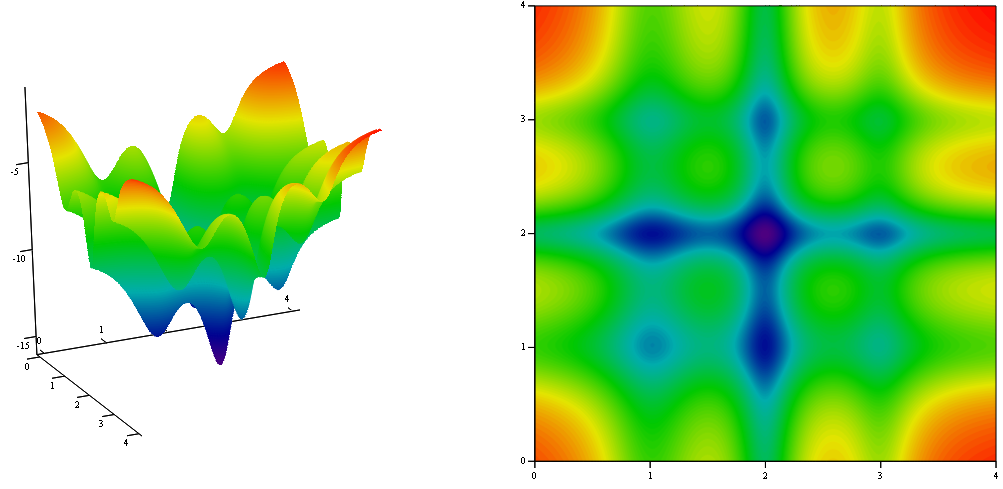
\includegraphics [scale=0.5] {MHL_TestFunction_AdditivePotential}
  \caption{Аддитивная потенциальная функция} 
  \label{TestFunctions:img:MHL_TestFunction_AdditivePotentiale}  
\end{figure}

\subsection {Параметры для алгоритмов оптимизации}

\begin{tabularwide}
\textbf{Точность вычислений:} & $\varepsilon=0.01$. \\
\textbf{Число интервалов, на которые предполагается разбивать каждую компоненту вектора $\bar{x}$ в пределах своего изменения} (для алгоритмов дискретной оптимизации) : & $NumberOfParts_j=4095$ ($j=\overline{1,n}$). \\
\textbf{Для этого длина бинарной строки для $x_j$ координаты равна} (для алгоритмов бинарной оптимизации) : & $\left( k_2\right)_j=12$ ($j=\overline{1,n}$). \\
\end{tabularwide}

\textbf{Замечание:}  $NumberOfParts_j$ выбирается как минимальное число, удовлетворяющее соотношению:
\begin{equation*}
NumberOfParts_j=2^{\left( k_2\right)_j }-1\geq\dfrac{10\left( Right_j-Left_j\right) }{\varepsilon},\text{где } \left( k_2\right)_j \in \mathbb{N}, \left( j=\overline{1,n}\right).
\end{equation*}

\subsection {Основная задача и подзадачи}

\begin{tabularwide}
\textbf{Изменяемый параметр: } & $n$ --- размерность вещественного вектора. \\
\textbf{Значение в основной задаче:} & $n=2$.\\
\end{tabularwide}

\subsection {Нахождение ошибки оптимизации}

Пусть в результате работы алгоритма оптимизации за $N$ запусков мы нашли решения $\bar{x}_{submin}^k$ со значениями целевой функции $f\left( \bar{x}_{submin}^k\right) $ соответственно ($k=\overline{1,N}$). Используем три вида ошибок:

\textbf{Надёжность: }
\begin{equation*}
R = \dfrac{\sum_{k=1}^{N}S\left( \bar{x}_{submin}^k \right) }{N}, \text{ где}
\end{equation*}
\begin{equation*}
S\left( \bar{x}_{submin}^k \right)=\left\lbrace \begin{aligned} 1,& \text{ если } \left| \left( \bar{x}_{submin}^k \right)_j-\left( \bar{x}_{min} \right)_j\right|\leq\varepsilon, j=\overline{1,n};   \\ 0,& \text{ иначе}. \end{aligned}\right.
\end{equation*}

\textbf{Ошибка по входным параметрам:}
\begin{equation*}
E_x = \dfrac{\sum_{k=1}^{N} \left( \frac{\sqrt{\sum_{j=1}^{n}{\left( \left( \bar{x}_{submin}^k \right)_j-\left( \bar{x}_{min} \right)_j \right)}^2 }}{n} \right)  }{N}.
\end{equation*}

\textbf{Ошибка по значениям целевой функции: }
\begin{equation*}
E_f = \dfrac{\sum_{k=1}^{N} \left| f\left( \bar{x}_{submin}^k \right)-f\left( \bar{x}_{min} \right) \right|  }{N}.
\end{equation*}

\subsection {Свойства задачи}
\begin{tabularwide}
\textbf{Условной или безусловной оптимизации: } & Задача безусловной оптимизации. \\
\textbf{Одномерной или многомерной оптимизации: } & Многомерной: $ n $. \\
\textbf{Функция унимодальная или многоэкстремальная: } & Функция многоэкстремальная. \\
\textbf{Функция стохастическая или нет: } & Функция не стохастическая. \\
\textbf{Особенности: } & Нет. \\
\end{tabularwide}

\subsection {Реализация}

Реализация функции взята из библиотеки HarrixMathLibrary в разделе <<Тестовые функции для оптимизации>>, которую можно найти по адресу \href{https://github.com/Harrix/HarrixMathLibrary} {https://github.com/Harrix/HarrixMathLibrary}.

\begin{lstlisting}[caption=Код функции MHL\_TestFunction\_AdditivePotential]
double MHL_TestFunction_AdditivePotential(double x, double y)
{
/*
Функция двух переменных: аддитивная потенциальная функция.
Тестовая функция вещественной оптимизации.
Входные параметры:
 x - первая вещественная переменная;
 y - вторая вещественная переменная.
Возвращаемое значение:
 Значение тестовой функции в точке (x,y).
*/
double VMHL_Result;
double z1=-(1./((x-1.)*(x-1.)+0.2))-(1./(2.*(x-2.)*(x-2.)+0.15))-(1./(3.*(x-3.)*(x-3.)+0.3));
double z2=-(1./((y-1.)*(y-1.)+0.2))-(1./(2.*(y-2.)*(y-2.)+0.15))-(1./(3.*(y-3.)*(y-3.)+0.3));
VMHL_Result=z1+z2;
return VMHL_Result;
}
\end{lstlisting}

\subsection {Ссылки}

Данная функция приводится в следующих источниках:

\begin{enumerate}
\item \cite[стр. 33]{book:Semenkin2007} ---  \href{http://files.lib.sfu-kras.ru/ebibl/umkd/22/u_lectures.pdf}{Эволюционные методы моделирования и оптимизации сложных систем}.
\end{enumerate}